% kapitel4.tex
\chapter{Wagner-Struktur}
\label{cha:wagnerstruktur}

In diesem Kapitel soll Theorem \ref{eq:Theorem36} genauer betrachtet werden.
Zunächst werden einige Baumstrukturen eingeführt, die den $3$-Zusammenhang herstellen können.
Anschließend werden \dd-Separatoren behandelt und eine Formulierung des Theorems von Wagner, das in Theorem \ref{eq:Theorem36} benutzt wurde, vorgestellt.

\section{$2$-Zusammenhang}

\begin{figure}[H]
  \centering
  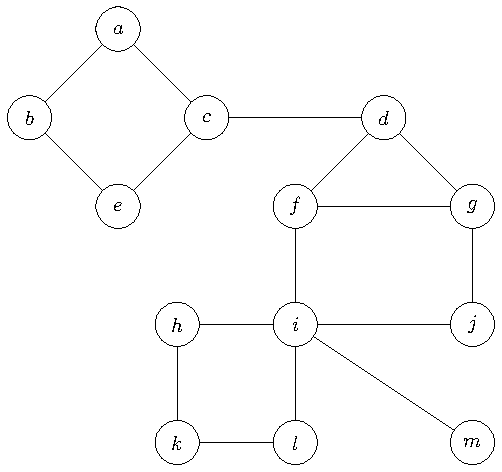
\includegraphics[width=10cm,keepaspectratio]{bilder/1-Block-Tree1.pdf}
  \caption{Ein nicht $2$-zusammenhängender Graph $G_1$.}
  \label{fig:1-Block-Tree1}
\end{figure}
\begin{definition}[\cite{BoM08}]
  Als \emph{Block} eines Graphen $G$ wird jeder seiner maximalen Teilgraphen bezeichnet, der keinen $1$-Separator enthält und für dessen Knotenmenge $V'$ gilt: $\vert V' \vert \geq 2$.
  Je zwei Blöcke haben maximal einen gemeinsamen Knoten, der einen $1$-Separator in $G$ bildet.
  Der \emph{Block-Cut Tree} $T_{bc} = (V_{bc}, E_{bc}, B)$ von $G$ ist ein Baum, der für jeden Block $b_v \in B$ von $G$ einen assoziierten Knoten $v \in V_{bc}$ besitzt.
  Sind $\{b_1, ..., b_k\} \subseteq B$ eine Menge von Blöcken, sodass alle den gleichen gemeinsamen Knoten $c$ haben, dann gibt es die Kanten $(b_i, b_j) \in E_{bc}$ für $1 \leq i \leq k$, $j \in [1, k]$, $i \neq j$.
  Dadurch ist $b_j$ ein beliebig, aber fester Block, der adjazent zu allen $b_i \in \{b_1, ..., b_k\}$ außer sich selbst ist.
\end{definition}
Als Beispiel wird in \Abb \ref{fig:1-Block-Tree1} ein Graph mit dazugehörigem Block-Cut Tree in \Abb \ref{fig:1-Block-Tree2} gezeigt.
Die Knoten des Block-Cut Tree sind als durchgezogene Linien angegeben, in jedem dieser Knoten findet sich ein $2$-zusammenhängender Teilgraph aus $G_1$.
\begin{figure}[H]
  \centering
  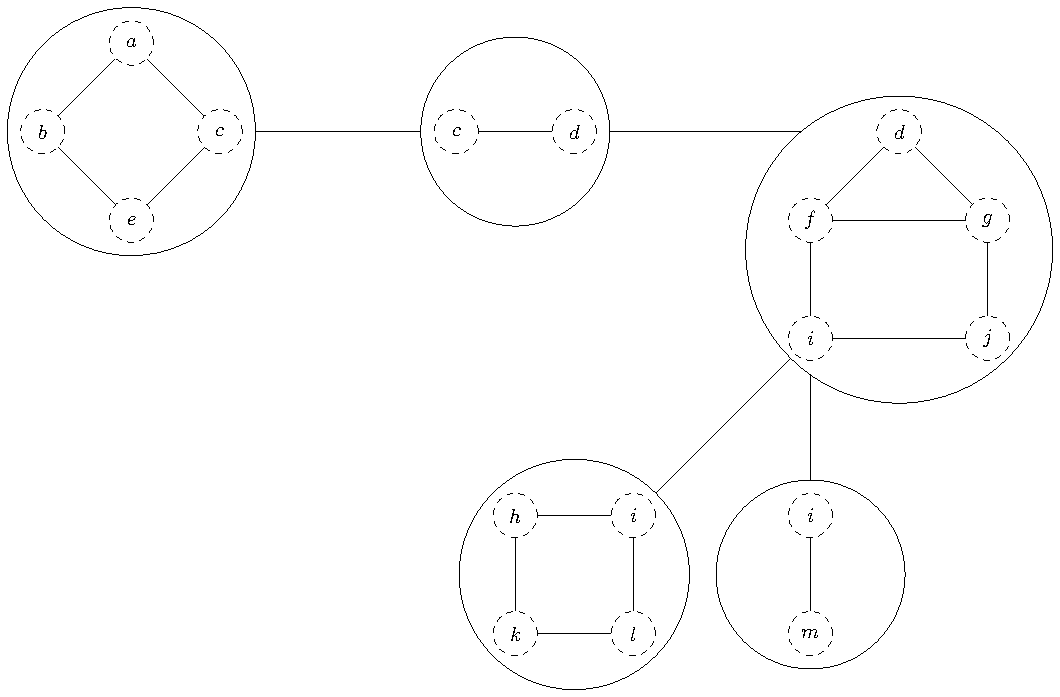
\includegraphics[width=\textwidth,height=\textheight,keepaspectratio]{bilder/1-Block-Tree2.pdf}
  \caption{Der Block-Cut Tree zu $G$ aus \Abb \ref{fig:1-Block-Tree1}.}
  \label{fig:1-Block-Tree2}
\end{figure}

Reed und Li stellen in \cite{ReL} und \cite{ReL08} Erweiterungen zum Block-Cut Tree vor, die für $1$-, $2$- und \dd-Separatoren definiert sind.
Der \emph{1-Block-Tree} unterscheidet sich im Wesentlichen vom Block-Cut Tree dadurch, dass für $1$-Separatoren zusätzliche Knoten im Baum angelegt werden.

\begin{definition}[\cite{ReL}]
  Ein \emph{1-Block-Tree} ist ein Baum $T = (V_T, E_T, \mathcal{G})$ für einen zusammenhängenden Graphen $G$.
  $V_T$ ist die Menge der Knoten, $E_T$ die der Kanten.
  Die Menge $\mathcal{G} = \{G_t\}_{t \in V_T}$ hat folgende Eigenschaften:
  \begin{itemize}
    \item Für alle Knoten $t \in V_T$ ist $G_t$ ein Graph.
    \item Ist $G$ $2$-zusammenhängend, hat der $1$-Block-Tree einen einzelnen Knoten $t$ mit $G_t = G$.
    \item Andernfalls gibt es einen als \emph{Cliquenknoten} bezeichneten $t \in V_T$:
    \begin{itemize}
      \item Ist $c$ ein $(1, j)$-Separator in $G$ für $j \geq 2$, dann ist $G_t = G(c)$.
      \item Seien $A_1, ..., A_j$ die augmentierten Komponenten definiert durch $G - c$.
            Dann gibt es $T_1, ..., T_j$ Teilbäume in $T - t$, sodass $T_i$ ein $1$-Block-Tree für $G_i = A_i$ ist.
      \item Für jeden $t_i \in V_T$, der $c$ als Teilgraph enthält, gibt es eine Kante $(t, t_i) \in E_T$.
    \end{itemize}
    \item Jeder Knoten, der kein Cliquenknoten ist, wird als \emph{Blockknoten} bezeichnet.
  \end{itemize}
\end{definition}
Sind $T_{bc}$ der Block-Cut-Tree und $T_1$ der $1$-Block-Tree für einen Graphen $G$, dann gibt es für jeden $v \in V_{bc}$ mit assoziiertem Block $b_v \in B$ einen Blockknoten $t \in V_T$, dessen Graph $G_t$ isomorph zu $b_v$ ist.
Ein Beispiel findet sich in \Abb \ref{fig:1-Block-Tree3}.
\begin{figure}[H]
  \centering
  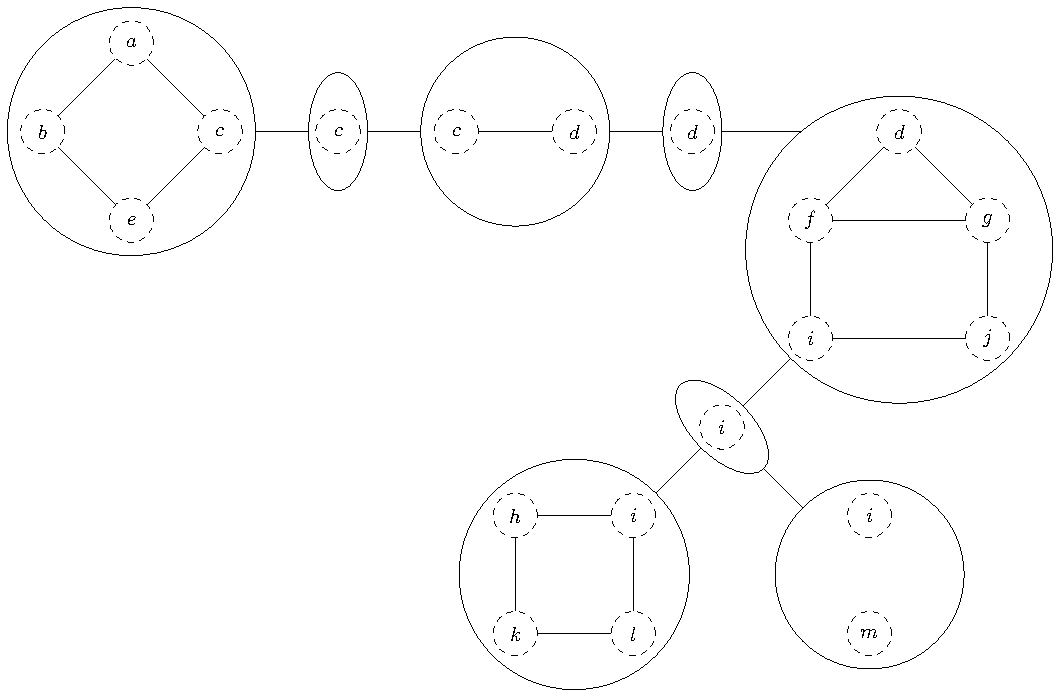
\includegraphics[width=\textwidth,height=\textheight,keepaspectratio]{bilder/1-Block-Tree3.pdf}
  \caption{Der $1$-Block-Tree zu $G$ aus \Abb \ref{fig:1-Block-Tree2}.
           Die Cliquenknoten sind ovalförmig dargestellt.}
  \label{fig:1-Block-Tree3}
\end{figure}


\section{$3$-Zusammenhang}

Nachdem durch Block-Cut Trees \bzw $1$-Block-Trees der $2$-Zusammenhang in allen Blockknoten hergestellt wurde, können die darin enthaltenen Teilgraphen jeweils als Eingabe für einen SPQR-Baum genutzt werden, um $3$-zusammenhängende Komponenten zu erzeugen.
Die folgende Definition dazu ist \cite{GuM00} entnommen.

\begin{figure}[H]
  \centering
  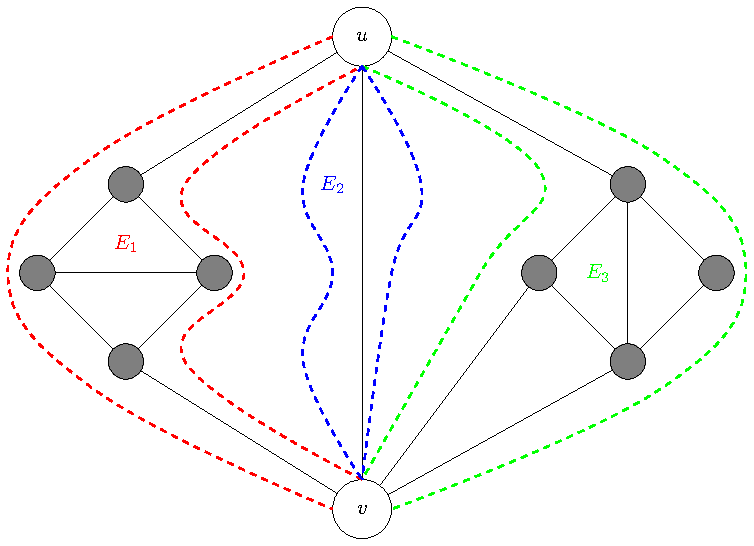
\includegraphics[width=\textwidth,height=\textheight,keepaspectratio]{bilder/Split-Kantenmengen.pdf}
  \caption{Unterteilung der Kanten in drei Mengen $E_1$, $E_2$ und $E_3$ anhand des Split Pairs $\{u, v\}$.}
  \label{fig:Split-Kantenmengen}
\end{figure}

\begin{definition}
  Sei $G = (V, E)$ ein $2$-zusammenhängender Graph.
  Als \emph{Split Pair} $\{u, v\}$ wird entweder ein adjazentes Knotenpaar oder ein $2$-Separator bezeichnet, ein \emph{maximales Split Pair} $\{s, t\}$ für $\{u, v\}$ teilt den Graphen so auf, dass $u$, $v$, $s$, und $t$ in einer $3$-zusammenhängenden Komponente liegen.
  Eine \emph{Split Component} für ein Split Pair ist entweder eine Kante zwischen diesem oder der maximale Teilgraph, für den es kein Split Pair mehr ist.
  Ein Split Pair teilt die Kanten des Graphen in die Mengen $E_1, ..., E_k$, sodass eine Menge $E_i$ alle Pfade enthält, die $u$ oder $v$ höchstens als Endpunkte haben.
  Dabei enthält $E_i$ entweder einen Teilgraphen von $G$, der nur die beiden Knoten enthält, oder einen, für den das Split Pair kein $2$-Separator ist.
  Eine Skizze dazu findet sich in \Abb \ref{fig:Split-Kantenmengen}.
  Der SPQR-Baum $T_{SPQR}$ von $G$ ist ein Baum, der $G$ anhand von jedem Split Pair $\{u, v\}$ rekursiv in Minoren aufteilt, die mit den Knoten des Baumes assoziiert und mit \emph{S}, \emph{P}, \emph{Q} oder \emph{R} markiert werden:
  \begin{itemize}
    \item \textbf{Q}: Tritt der Randfall auf, dass $G$ nur eine einzige Kante $(u, v)$ besitzt, dann enthält der SPQR-Baum einen einzelnen Q-Knoten, der auf $G$ verweist.
    \item \textbf{P}: Entstehen durch das Split Pair die Kantenmengen $E_1, ..., E_k$ mit $k \geq 3$, dann wird ein P-Knoten hinzugefügt.
                      Der assoziierte Graph besteht aus dem Split Pair sowie $k$ Kanten zwischen diesem.
    \item \textbf{S}: Andernfalls teilen $u$ und $v$ die Kanten in zwei Mengen, sodass es eine Kante $(u, v) \in E$ und einen weitere Pfad gibt, der das Split Pair verbindet.
                      Der hinzugefügte S-Knoten enthält die Kante und den Pfad.
    \item \textbf{R}: Tritt keiner der obigen Fälle ein, dann seien $\{s_1, t_1\}, ..., \{s_k, t_k\}$ für $k \geq 1$ die maximalen Split Pairs für ${u, v}$ und $G_i$ für alle $1 \leq i \leq k$ die Vereinigung aller Split Components für $\{u, v\}$ außer der, die die Kante $(u, v)$ enthält.
                      Der neue R-Knoten enthält $G$, wobei jeder Teilgraph $G_i$ durch die Kante $(s_i, t_i)$ ersetzt wird.
  \end{itemize}
\end{definition}

\ \\

\begin{figure}[H]
  \centering
  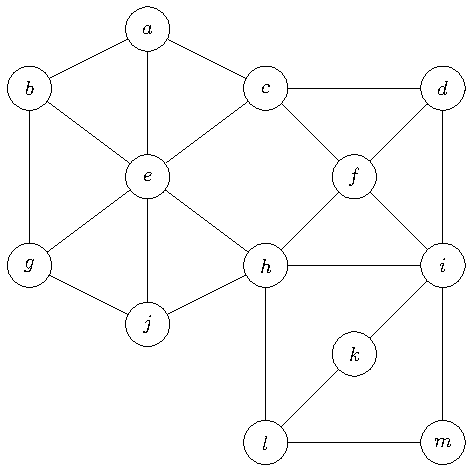
\includegraphics[width=10cm]{bilder/2-Block-Tree1.pdf}
  \caption{Ein $2$-zusammenhängender Graph $G_2$.}
  \label{fig:2-Block-Tree1}
\end{figure}

\newpage

\begin{figure}[H]
  \centering
  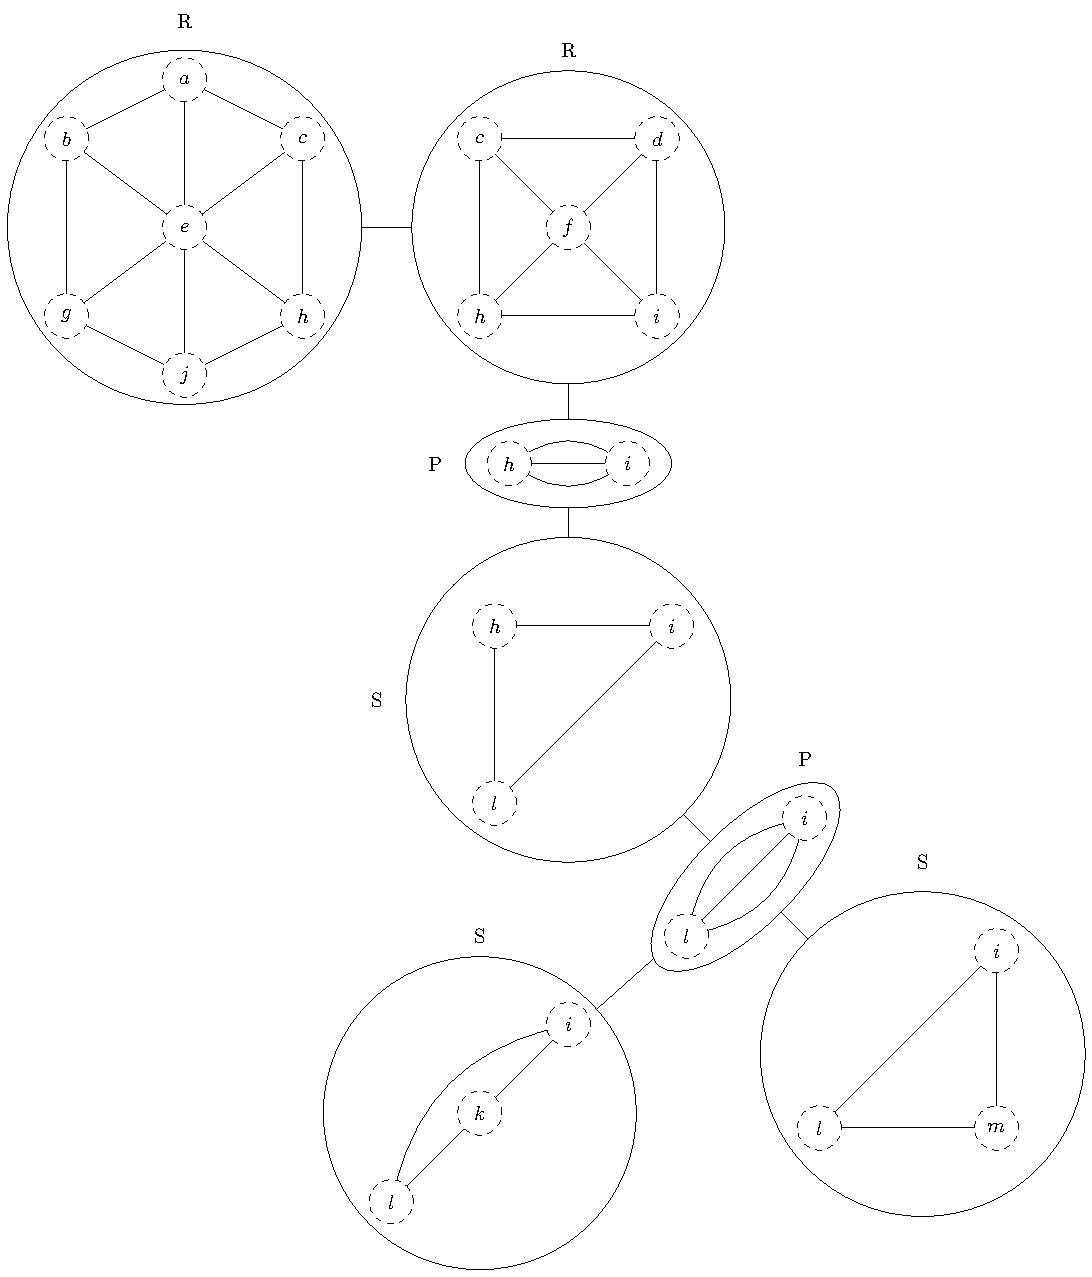
\includegraphics[width=\textwidth,height=\textheight,keepaspectratio]{bilder/SPQR-Tree.pdf}
  \caption{SPQR Baum zum Graphen $G_2$ aus \Abb \ref{fig:2-Block-Tree1}.}
  \label{fig:SPQR-Tree}
\end{figure}

Zu dem Graphen in \Abb \ref{fig:2-Block-Tree1} ist in \Abb \ref{fig:SPQR-Tree} der zugehörige SPQR Baum skizziert.
Besonders interessant sind die R-Knoten, die $3$-zusammenhängende Minoren von $G_2$ sind.
Zwar gilt das auch für die drei S-Knoten, allerdings sind Kreise im Allgemeinen nicht $3$-zusammenhängend, aber immer planar.

Analog zum $1$-Block-Tree stellen Li und Reed in \cite{ReL08} den \emph{2-Block-Tree} vor.
Er unterscheidet sich deutlich vom SPQR-Baum, enthält aber ebenfalls $3$-zusammenhängende Minoren.

\begin{definition}[\cite{ReL08}]
Ein \emph{2-Block-Tree} ist ein Baum $T = (V_T, E_T, \mathcal{G})$ für einen $2$-zusammenhängenden Graphen $G$.
$V_T$ ist die Menge der Knoten, $E_T$ die der Kanten.
Die Menge $\mathcal{G} = \{G_t\}_{t \in V_T}$ hat folgende Eigenschaften:
\begin{itemize}
  \item Für alle Knoten $t \in V_T$ ist $G_t$ ein Graph.
  \item Ist $G$ $3$-zusammenhängend, hat der $2$-Block-Tree einen einzelnen Knoten $t$ mit $G_t = G$.
  \item Andernfalls gibt es einen Cliquenknoten $t \in V_T$:
  \begin{itemize}
    \item Ist $C = \{c_1, c_2\}$ ein $(2, j)$-Separator in $G$ für $j \geq 2$, dann ist $G_t = G(C)$.
          Es werden Kanten zu $G_t$ hinzugefügt, bis $G_t$ eine Clique ist.
    \item Seien $A_1, ..., A_j$ die augmentierten Komponenten definiert durch $G - C$.
          Dann gibt es $T_1, ..., T_j$ Teilbäume in $T - t$, sodass $T_i$ ein $2$-Block-Tree für $G_i = A_i$ ist.
    \item Für jeden $t_i \in V_T$, der $C$ als Teilgraph enthält, gibt es eine Kante $(t, t_i) \in E_T$.
  \end{itemize}
  \item Jeder Knoten, der kein Cliquenknoten ist, ist ein Blockknoten.
\end{itemize}
\end{definition}

Ein $2$-Block-Tree zu $G_2$ aus \Abb \ref{fig:2-Block-Tree1} ist in \Abb \ref{fig:2-Block-Tree2} zu sehen.
Es ist zu beobachten, dass Knoten wie etwa $h$ oder $i$ Teil mehrerer Separatoren sein können und somit nicht nur in mehreren Block-, sondern auch in mehreren Cliquenknoten enthalten sind.

\newpage

\begin{figure}[H]
  \centering
  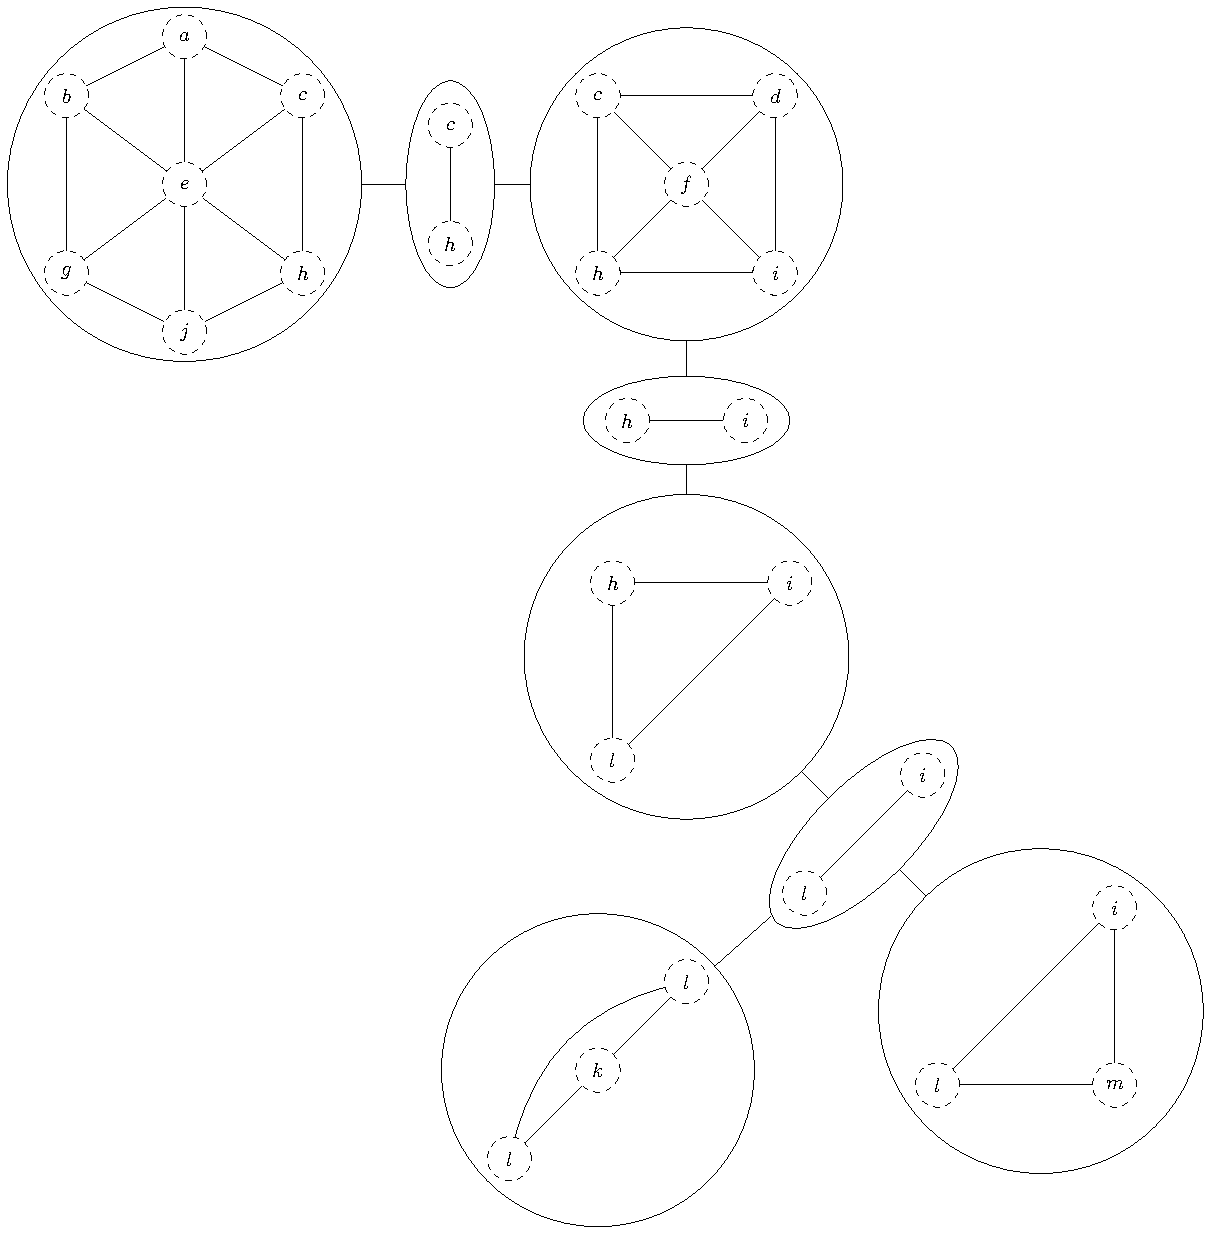
\includegraphics[width=\textwidth,height=\textheight,keepaspectratio]{bilder/2-Block-Tree2.pdf}
  \caption{$2$-Block-Tree zum Graphen aus \Abb \ref{fig:2-Block-Tree1}.
           Die Cliquenknoten sind ovalförmig dargestellt und enthalten immer genau zwei Knoten, alle übrigen sind Blockknoten.}
  \label{fig:2-Block-Tree2}
\end{figure}

\newpage

\section{\dd-Separatoren}

Letztlich wird in \cite{ReL08} eine weitere Baumstruktur für \dd-Separatoren eingeführt:

\begin{definition}[\cite{ReL08}]
Ein \emph{(3, 3)-Block-Tree} ist ein Baum $T = (V_T, E_T, \mathcal{G})$ für einen $3$-zusammenhängenden Graphen $G$.
$V_T$ ist die Menge der Knoten, $E_T$ die der Kanten.
Die Menge $\mathcal{G} = \{G_t\}_{t \in V_T}$ hat folgende Eigenschaften:
\begin{itemize}
  \item Für alle Knoten $t \in V_T$ ist $G_t$ ein Graph.
  \item Hat $G$ keinen \dd-Separator, hat der \dd-Block-Tree einen einzelnen Knoten $t$ mit $G_t = G$.
  \item Andernfalls gibt es einen Cliquenknoten $t \in V_T$:
  \begin{itemize}
    \item Ist $C = \{c_1, c_2, c_3\}$ ein $(3, j)$-Separator in $G$ für $j \geq 3$, dann ist $G_t = G(C)$.
          Es werden Kanten zu $G_t$ hinzugefügt, bis $G_t$ eine Clique ist.
    \item Seien $A_1, ..., A_j$ die augmentierten Komponenten definiert durch $G - C$.
          Dann gibt es $T_1, ..., T_j$ Teilbäume in $T - t$, sodass $T_i$ ein \dd-Block-Tree für $G_i = A_i$ ist.
    \item Für jeden $t_i \in V_T$, der $C$ als Teilgraph enthält, gibt es eine Kante $(t, t_i) \in E_T$.
  \end{itemize}
  \item Jeder Knoten, der kein Cliquenknoten ist, ist ein Blockknoten.
\end{itemize}
\end{definition}

Ein Beispiel ist in \Abb \ref{fig:33-Block-Tree} skizziert.

\newpage

\begin{figure}[H]
  \centering
  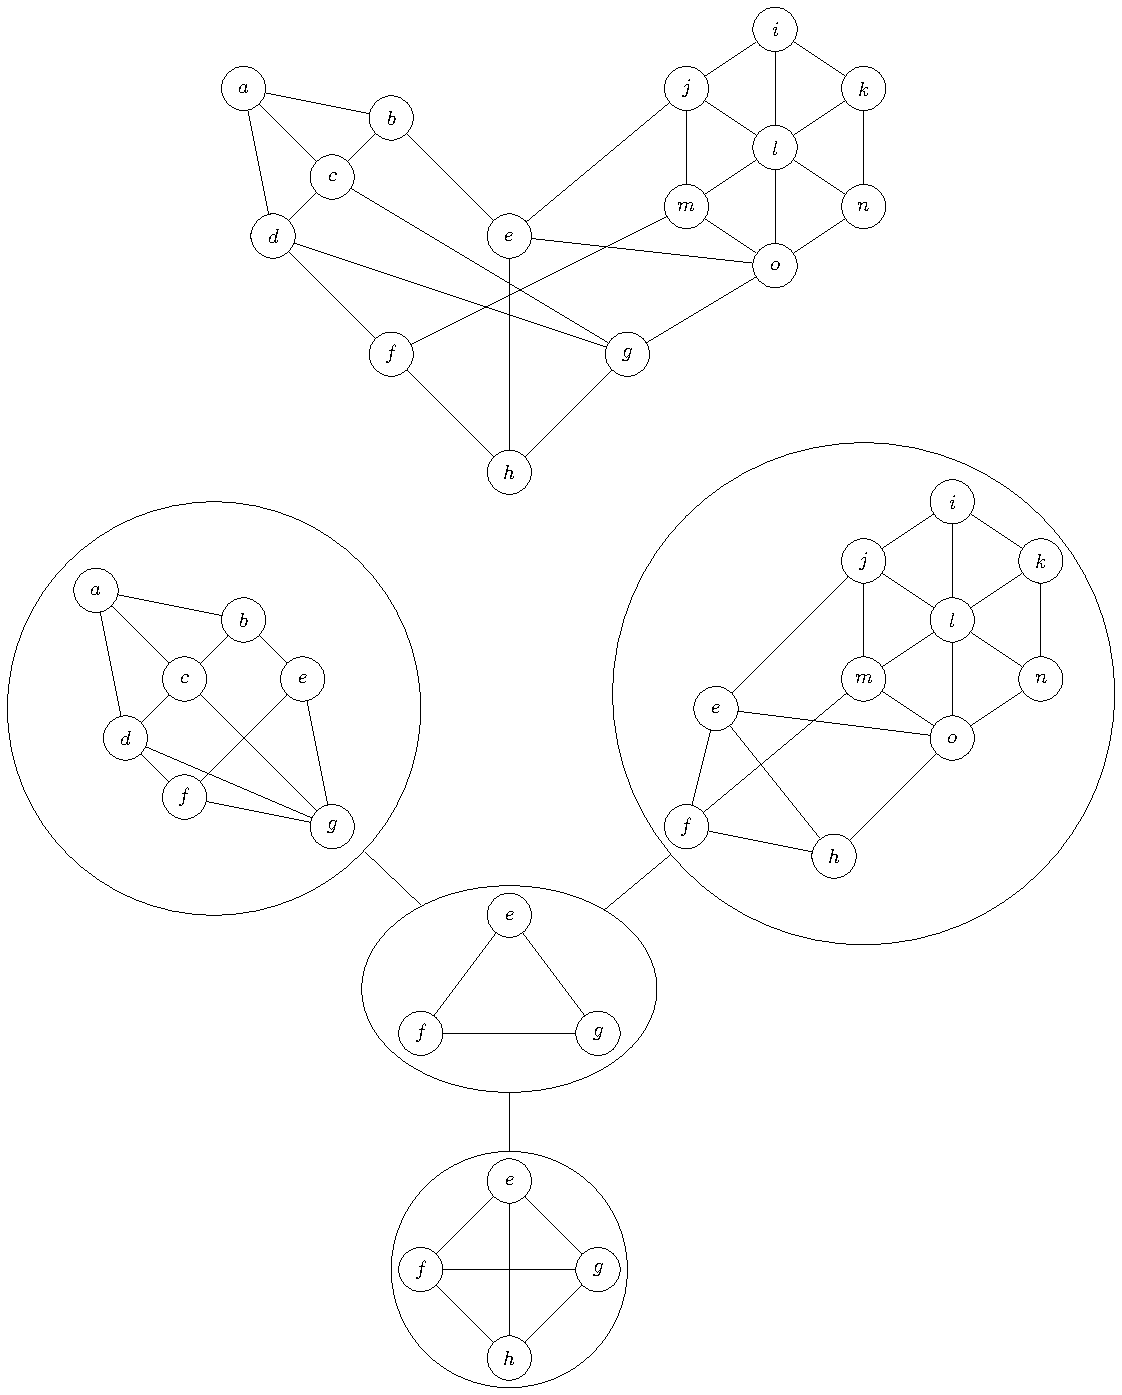
\includegraphics[width=\textwidth,height=\textheight,keepaspectratio]{bilder/33-Block-Tree.pdf}
  \caption{Ein $3$-zusammenhängender Graph mit dazugehörigem \dd-Block-Tree.
           Der Separator wird durch $\{e, f, g\}$ gebildet.
           Es ist zu sehen, dass der Eingabegraph nicht planar ist, da ein \kdd-Minor enthalten ist.
           Die Blockknoten enthalten jedoch alle planare Minoren des ursprünglichen Graphs.}
  \label{fig:33-Block-Tree}
\end{figure}


\section{Wagner-Struktur}
\begin{definition}[\cite{ReL}]\label{eq:WagnerStruktur}
  Sei $G$ ein zusammenhängender Graph.
  Die \emph{Wagner-Struktur} von $G$ ist ein $1$-Block-Tree $R = (V, E, \mathcal{G})$ und ein $2$-Block-Tree $S_r = (V_r, E_r, \mathcal{G}_r)$ für jeden Blockknoten $r \in V$ und ein \dd-Block-Tree $T_{s_t} = (V_{s_t}, E_{s_t}, \mathcal{G}_{s_t})$ für jeden Blockknoten $s \in V_r, r \in V$.
\end{definition}

Dadurch kann das Theorem von Wagner wie folgt formuliert werden:

\begin{theorem}[\cite{Wag37}]\label{eq:TheoremWagner}
  Ein zusammenhängender Graph enthält genau dann keinen \kf-Minor, wenn für ihn eine Wagner-Struktur existiert, sodass für alle \dd-Block-Trees $T_{s_t} = (V_{s_t}, E_{s_t}, \mathcal{G}_{s_t}$ gilt: Jeder Graph $G \in \mathcal{G}_{s_t})$ ist entweder planar oder isomorph zu $W$.
\end{theorem}

Trifft Theorem \ref{eq:TheoremWagner} auf die Wagner-Struktur eines Graphen $G$ nicht zu, wird sie als \emph{ungültig} bezeichnet und $G$ enthält einen \kf-Minor.
Ebenso werden \dd-Block-Trees als ungültig bezeichnet, wenn in ihnen ein \kf-Minor gefunden wird.
Eine Wagner-Struktur kann ebenfalls für einen nicht-zusammenhängenden Graphen $G$ aufgebaut werden.
In dem Fall besteht sie aus einem Wald, der einen $1$-Block-Tree für jede Zusammenhangskomponente von $G$ hat.

Als Beispiel ist dazu in \Abb \ref{fig:WagnerStruktur1} ein Graph $G$ zu sehen, der nicht planar ist, aber keinen \kf-Minor enthält.
In \Abb \ref{fig:WagnerStruktur2} sind die $3$-zusammenhängenden Graphen $G_1$, $G_2$, $G_3$, $G_4$, $G_5$ und $G_6$ abgebildet, von denen ebenfalls keiner einen \kf-Minor enthält.
Außerdem ist $G_6$ nicht planar.
Einige Cliquen sind in beiden Abbildungen mit je einer Farbe hervorgehoben, sodass durch Cliquen-Summen ein Graph $G'$ erzeugt werden kann, der $G$ als Teilgraphen enthält.
In \Abb \ref{fig:WagnerStruktur3} ist die Wagner-Struktur zu $G$ skizziert.
Der $1$-Block-Tree wurde nicht eingezeichnet, da er aufgrund des $2$-Zusammenhangs von $G$ aus nur einem Blockknoten besteht.
Foglich existiert ein einzelner $2$-Block-Tree, der aus blauen Knoten und Kanten besteht.
Für jeden seiner Blockknoten existiert ein \dd-Block-Tree (rot).
Es kann beobachtet werden, dass die Cliquenknoten aller Block-Trees genau die farblich markierten Cliquen aus \Abb \ref{fig:WagnerStruktur2} enthalten und in $G$ Separatoren bilden.
Außerdem ist zu sehen, dass die Blockknoten aller \dd-Block-Trees entweder planar oder isomorph zu $W$ sind.
Daraus folgt, dass $G$ keinen \kf-Minor enthält.

\newpage

\begin{figure}[H]
  \centering
  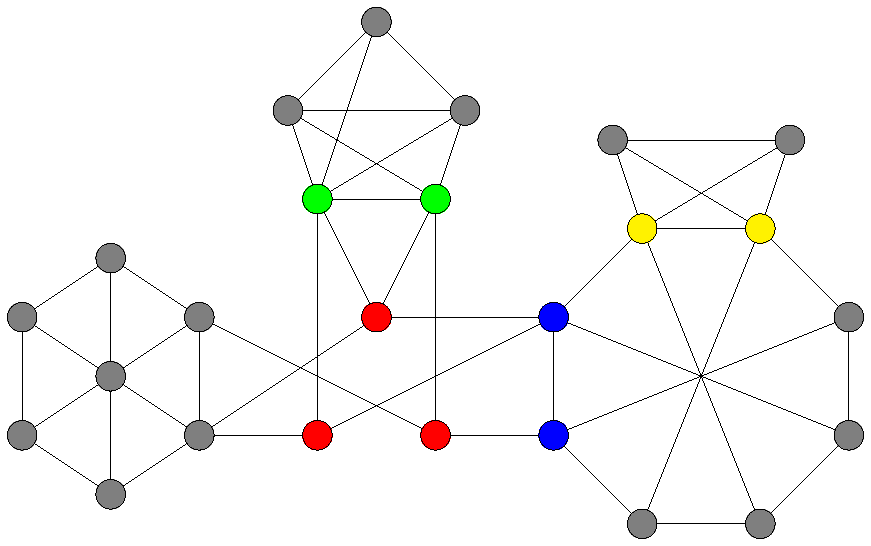
\includegraphics[width=\textwidth,height=\textheight,keepaspectratio]{bilder/WagnerTheorem1.pdf}
  \caption{Ein nicht-planarer Graph $G$, der keinen \kf-Minor enthält.}
  \label{fig:WagnerStruktur1}
\end{figure}

\begin{figure}[H]
  \centering
  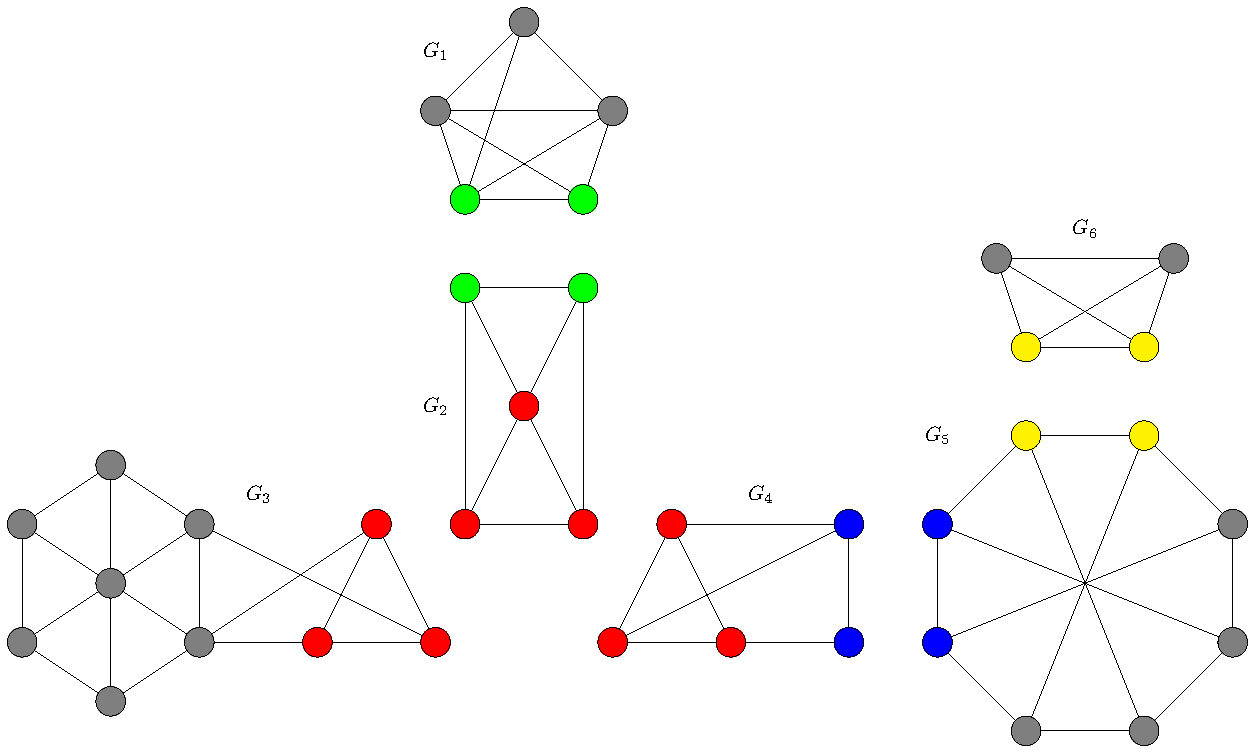
\includegraphics[width=\textwidth,height=\textheight,keepaspectratio]{bilder/WagnerTheorem2.pdf}
  \caption{Mehrere Graphen, die planar oder isomorph zu $W$ sind.}
  \label{fig:WagnerStruktur2}
\end{figure}

\begin{figure}[H]
  \centering
  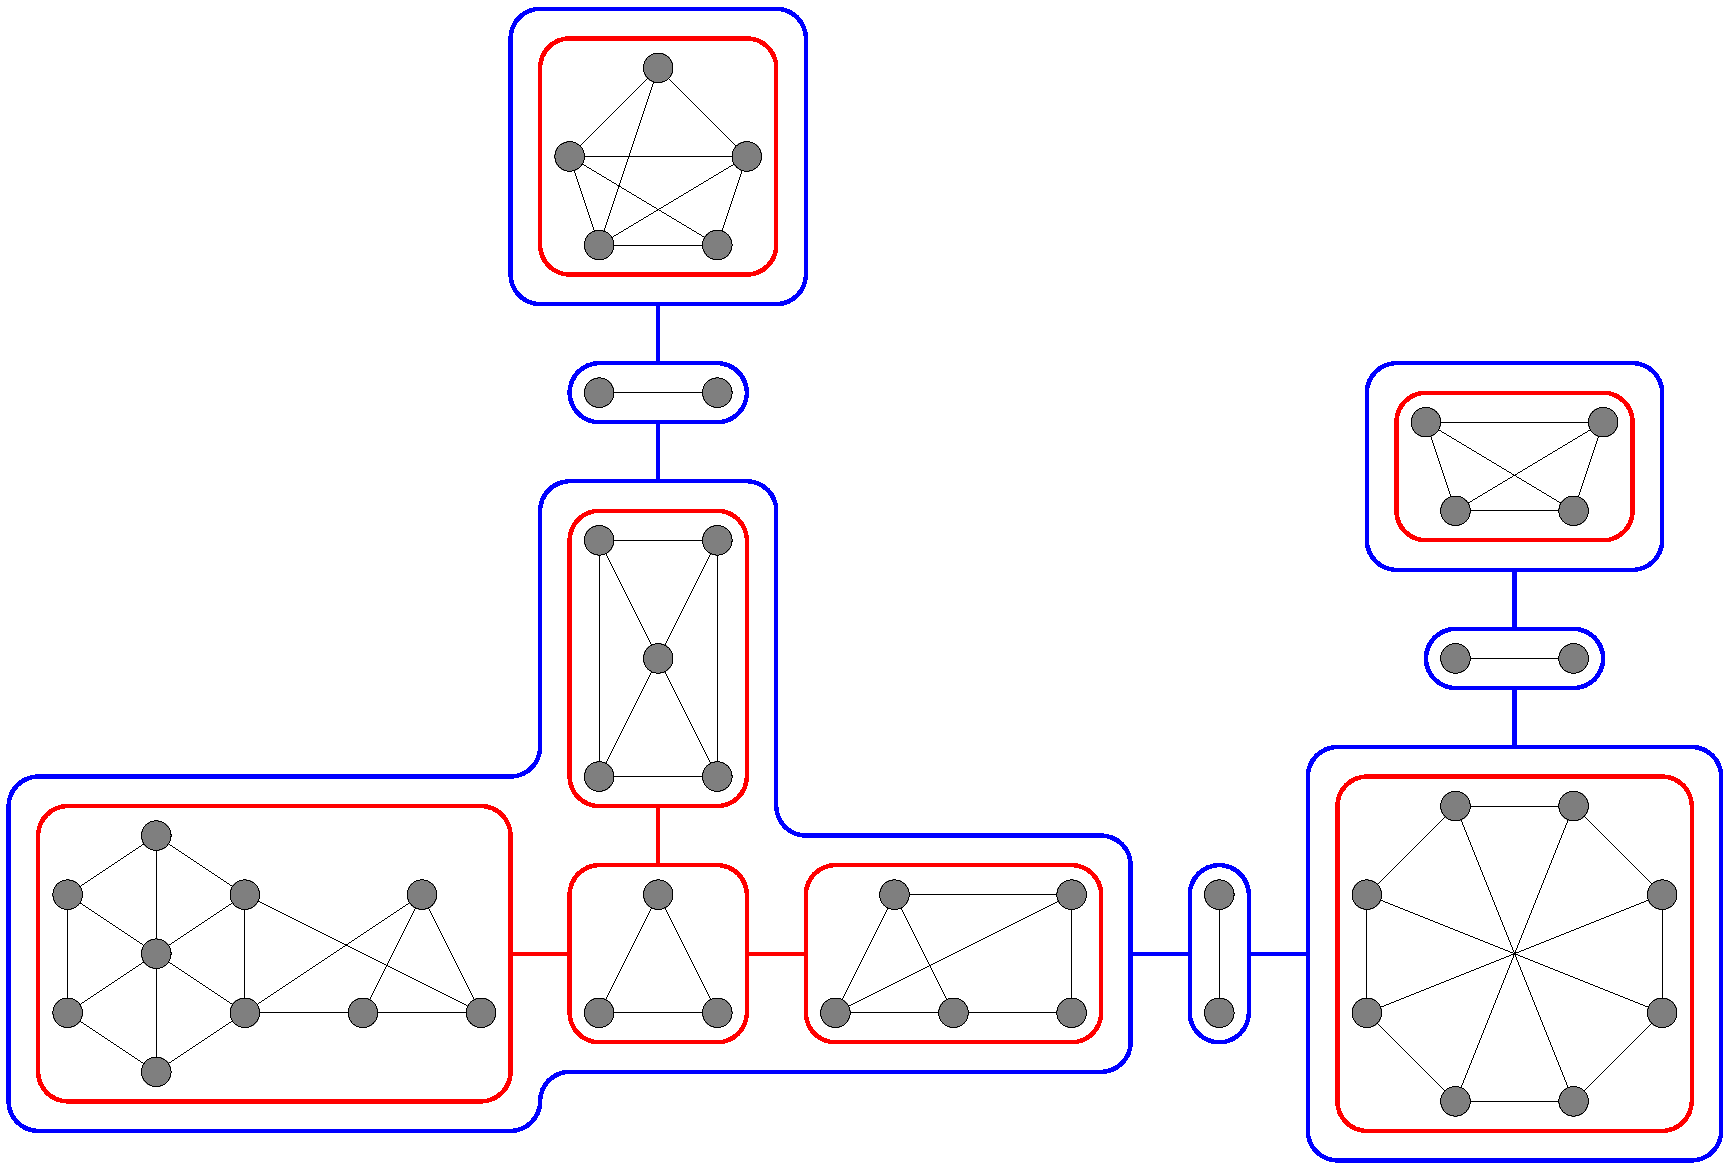
\includegraphics[width=\textwidth,height=\textheight,keepaspectratio]{bilder/WagnerTheorem3.pdf}
  \caption{Wagner-Struktur von $G$ aus \Abb \ref{fig:WagnerStruktur1}.
           Da $G$ bereits $2$-zusammenhängend ist, enthält der $1$-Block-Tree einen einzelnen Blockknoten für den kompletten Graphen und wurde nicht eingezeichnet.
           Die Knoten und Kanten des $2$-Block-Trees sind blau, die der \dd-Block-Trees rot hervorgehoben.}
  \label{fig:WagnerStruktur3}
\end{figure}
